\let\negmedspace\undefined
\let\negthickspace\undefined
\documentclass[journal]{IEEEtran}
\usepackage[a5paper, margin=10mm, onecolumn]{geometry}
%\usepackage{lmodern} % Ensure lmodern is loaded for pdflatex
\usepackage{tfrupee} % Include tfrupee package

\setlength{\headheight}{1cm} % Set the height of the header box
\setlength{\headsep}{0mm}     % Set the distance between the header box and the top of the text

\usepackage{gvv-book}
\usepackage{gvv}
\usepackage{cite}
\usepackage{amsmath,amssymb,amsfonts,amsthm}
\usepackage{algorithmic}
\usepackage{graphicx}
\usepackage{textcomp}
\usepackage{xcolor}
\usepackage{txfonts}
\usepackage{listings}
\usepackage{enumitem}
\usepackage{mathtools}
\usepackage{gensymb}
\usepackage{comment}
\usepackage[breaklinks=true]{hyperref}
\usepackage{tkz-euclide} 
\usepackage{listings}
% \usepackage{gvv}                                        
\def\inputGnumericTable{}                                 
\usepackage[latin1]{inputenc}                                
\usepackage{color}                                            
\usepackage{array}                                            
\usepackage{longtable}                                       
\usepackage{calc}                                             
\usepackage{multirow}                                         
\usepackage{hhline}                                           
\usepackage{ifthen}                                           
\usepackage{lscape}
\usepackage{circuitikz}
\tikzstyle{block} = [rectangle, draw, fill=blue!20, 
    text width=4em, text centered, rounded corners, minimum height=3em]
\tikzstyle{sum} = [draw, fill=blue!10, circle, minimum size=1cm, node distance=1.5cm]
\tikzstyle{input} = [coordinate]
\tikzstyle{output} = [coordinate]
\begin{document}
\textbf{Question:}

If \( D\left(-\frac{1}{2}, \frac{5}{2}\right), \quad E(7,3), \quad F\left(\frac{7}{2}, \frac{7}{2}\right) \) are the midpoints of the sides of \(\triangle ABC\), find the area of \(\triangle ABC\).

\vspace{1em}

\textbf{Solution:}

Let the position vectors of vertices \(A, B, C\) be \(\vec{A}, \vec{B}, \vec{C}\).

Using midpoint relations:

\[
\vec{D} = \frac{\vec{B} + \vec{C}}{2}, \quad \vec{E} = \frac{\vec{C} + \vec{A}}{2}, \quad \vec{F} = \frac{\vec{A} + \vec{B}}{2}
\]

Rearranging,

\[
\vec{A} - \vec{B} = 2(\vec{F} - \vec{D}), \quad \vec{A} - \vec{C} = 2(\vec{E} - \vec{D})
\]

The area of \(\triangle ABC\) is:

\[
\text{Area} = \frac{1}{2} \left\| (\vec{A} - \vec{B}) \times (\vec{A} - \vec{C}) \right\| = \frac{1}{2} \left\| 2(\vec{F} - \vec{D}) \times 2(\vec{E} - \vec{D}) \right\| = 2 \left\| (\vec{F} - \vec{D}) \times (\vec{E} - \vec{D}) \right\|
\]

Calculate the difference vectors as matrices:

\[
\vec{F} - \vec{D} =
\begin{pmatrix}
\frac{7}{2} \\
\frac{7}{2}
\end{pmatrix}
-
\begin{pmatrix}
-\frac{1}{2} \\
\frac{5}{2}
\end{pmatrix}
=
\begin{pmatrix}
4 \\
1
\end{pmatrix}
\]

\[
\vec{E} - \vec{D} =
\begin{pmatrix}
7 \\
3
\end{pmatrix}
-
\begin{pmatrix}
-\frac{1}{2} \\
\frac{5}{2}
\end{pmatrix}
=
\begin{pmatrix}
\frac{15}{2} \\
\frac{1}{2}
\end{pmatrix}
\]

The magnitude of their cross product is the determinant:

\[
\left\| (\vec{F} - \vec{D}) \times (\vec{E} - \vec{D}) \right\| = 
\left|
\begin{vmatrix}
4 & \frac{15}{2} \\
1 & \frac{1}{2}
\end{vmatrix}
\right| = \left| 4 \times \frac{1}{2} - 1 \times \frac{15}{2} \right| = |2 - 7.5| = 5.5
\]
 the area of \(\triangle ABC\) is:

\[
\text{Area} = 2 \times 5.5 = 11
\]

\[
\boxed{11}
\]

\begin{figure}
    \centering
    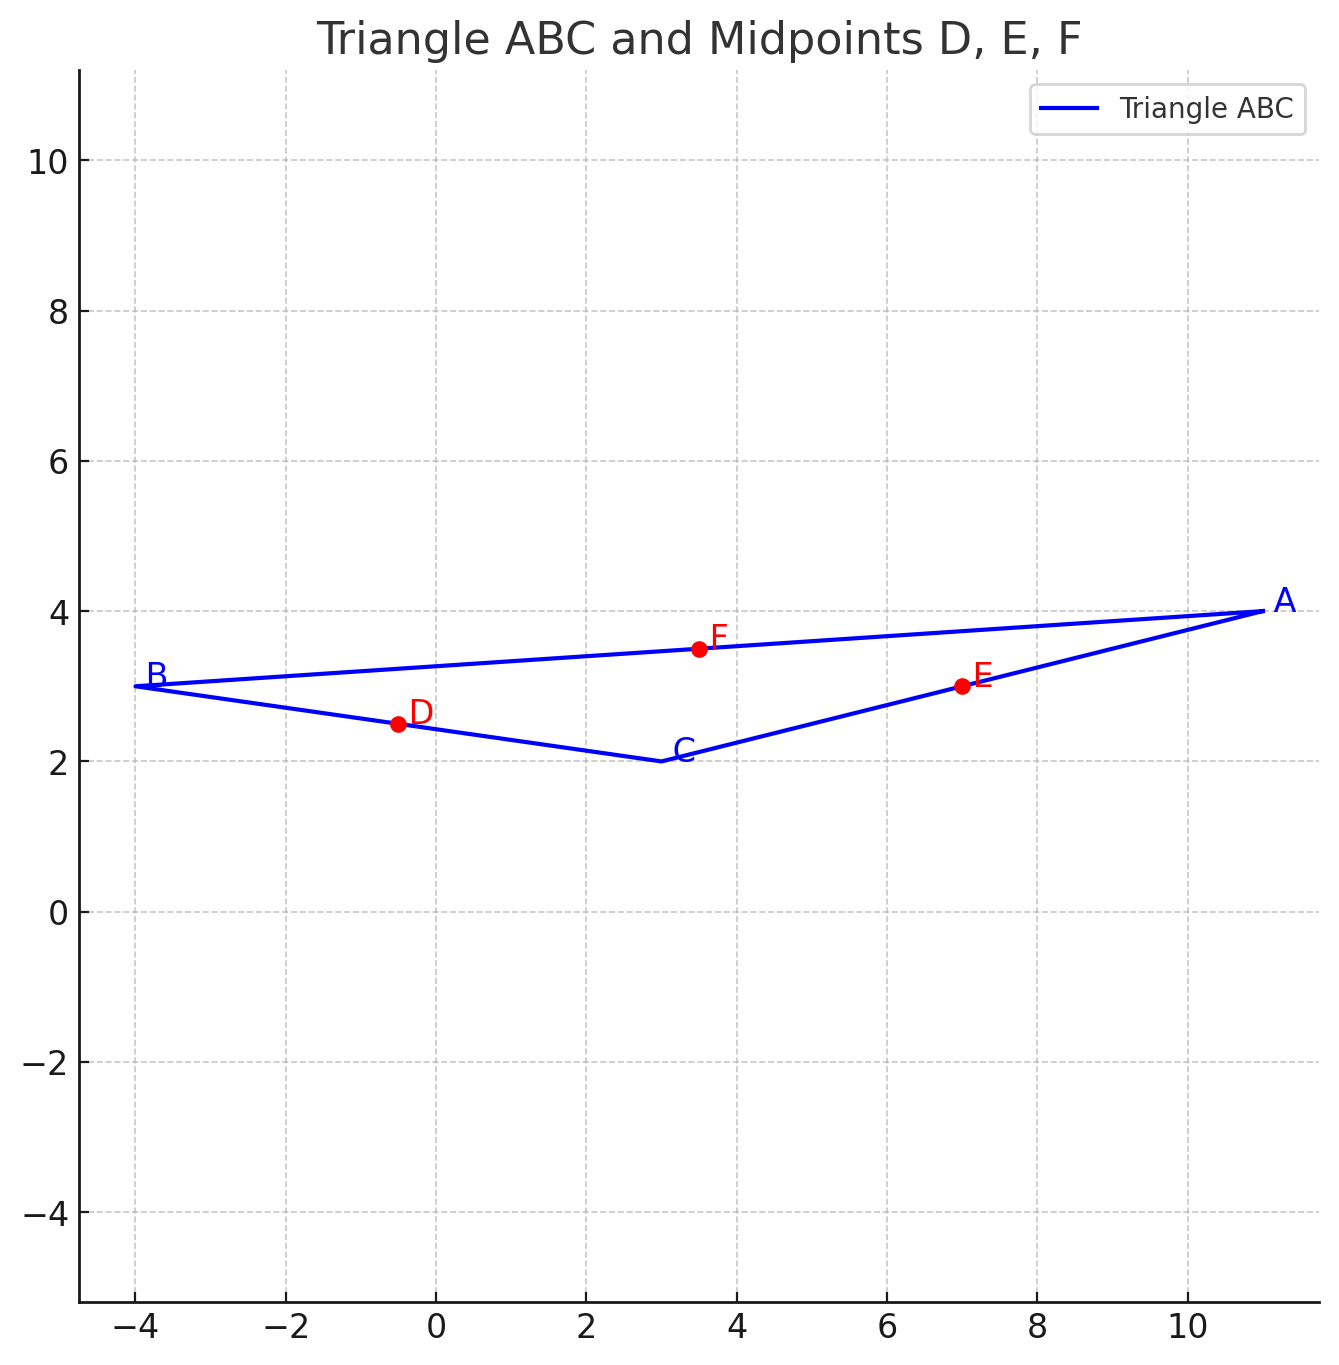
\includegraphics[width=1\linewidth]{figs/area.png}
    \caption{area}
    \label{fig:placeholder}
\end{figure}
\end{document}